% !TEX root = ../thesis.tex

\chapter{Syntetická časť}
\label{methodology}
V tejto časti si prejdeme konceptuálny návrh riešenia na predikciu víťazného tímu v profesionálnych e-sport zápasoch v hre League of Legends a bližšie sa pozrieme na metódy a hodnoty, ktoré budú potrebné pri jednotlivých fázach z návrhu riešenia a na finálnu tvorbu prototypu. 
\subsubsection{Konceptuálny návrh manipulácie s dátami}
Ako môžeme vidieť na obrázku \ref{koncept} manipuláciu dát sme rozdelili na 4 fázy plus testovanie a návrh používateľského rozhrania : 
 \begin{figure}[h!]
	
	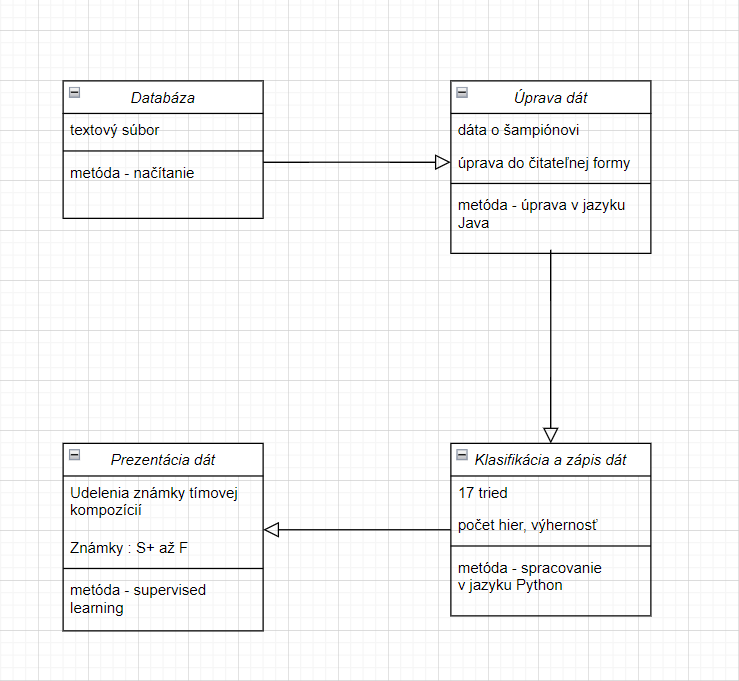
\includegraphics[width=.9\textwidth]{figures/koncept}
	\centering
	\caption{ Konceptuálny návrh riešenia \label{koncept}}
	
\end{figure}



\begin{enumerate}
	\item Prevziať potrebné dáta z hier cez databázu
	\item Upraviť ich do čitateľnej verzie pre umelú inteligenciu
	\item Spracovať a klasifikovať dáta na výpočet percentuálnej pravdepodobnosti na výhru a odskúšať prototyp
	\item Prepísať výsledky do čitateľnej formy pre zákazníkov
	\item Otestovať model a vizualizovať výsledky
\end{enumerate}

\section{Prevzatie dát z databáz}
V databázach bolo nielen veľké množstvo druhov dát, ale aj spôsobov, akým tieto dáta získať. Bola možnosť zobrať dáta zo všetkých hier, čiže aj neprofesionálnych alebo hier len z profesionálnych turnajov. Po dlhom uvažovaní a viacerých skúškach sme sa rozhodli použiť dáta iba z hier profesionálnych turnajov z celého sveta a to konkrétne z posledných 5 mesiacov. Dokopy je rôznych inštancií, ktoré berieme do úvahy, viac ako 250 000.

\subsection{Finálny druh dát}
Používané dáta budú mať 4 atribúty. Meno šampióna, pozícia v hre, počet hier, miera výhry vzhľadom na šampióna, s ktorým je v tíme. Tieto dáta budú v pozorovaní vzťahu medzi sebou v tíme. Lepšie povedané, budeme sa snažiť určiť, akú efektivitu má daný šampión, ak je sprevádzaný šampiónom z inej triedy. 

\section{Úprava dát}
Keďže databázy nie sú predpripravené na okamžité využitie pri umelej inteligencii, museli sme dáta prispôsobiť do podoby, ktoré python, konkrétne scikit learn, vie načítať. Dát je príliš veľa na ručnú úpravu, preto sme napísali kód v jave, ktorý načíta databázy, každé slovo dá do úvodzoviek, dá medzi ne čiarku a odstráni všetky tabulátory a medzery.

\section{Klasifikácia dát}
Vzhľadom na veľké množstvo rôznych šampiónov sme sa rozhodli rozdeliť ich na určité triedy podľa ich významu v hre a ich pozícii v tíme.
V hre je 5 pozícií a pre každú sme vybrali najčastejšie kategórie, do ktorých patria šampióni. Pri rozhodovaní sme mali pár otázok aj na 3 profesionálnych hráčov. Hráč Odoamne z Rumunska hraje na pozícii TOP za jeden z najlepších európskych tímov Rogue, v rozhovore povedal, že v jeho pozícií je dôležité vybrať šampióna, ktorý nie je veľmi slabý na začiatku hry a zároveň je dôležité, aby šampión podporoval svoj tím presne v tom, v čom je ich tím slabý. Druhý rozhovor bol s hráčom Selfmade zo Slovinska, ktorý hraje na pozícii JG za tím Vitality, on povedal, že aktuálne je dôležité, aby šampión v jeho pozície vedel rýchlo zabíjať tábory(6 rozdelených miest, kde zabíja monštrá za peniaze a obnovia sa dookola za 2 a pol až 5 minút). Tretí rozhovor bol s hráčom MikyX zo Slovinska, ktorý aktuálne hrá za tím Excel. MikyX hraje na pozícií SUP a povedal, že je veľmi ťažké predpovedať aký šampión bude dobrý do jeho pozície a že veľmi záleží od toho, čo vyberie oponent alebo jeho spoluhráči.  Tu sú triedy aj s krátkymi popismi :
\begin{enumerate}
	\item TOP - pozícia na vrchu mapy, väčšinou izolovaná až do neskorších fáz hry
	 \begin{itemize}
		\item laner - šampión, ktorý si zakladá na ich sile v prvých štádiách hry
		\item splitpusher - šampión, ktorý je rád izolovaný a rýchlo ničí veže
		\item teamfightdamage - šampión, ktorý exceluje v neskorších fázach hry a jeho primárnou prioritou je urobiť čo najväčšie poškodenie nepriateľským šampiónom počas tímového boja
		\item teamfightcc - skratka cc znamená crowd control, myslené ako udržanie nepriateľského šampióna v nehybnom stave, zatiaľ čo ho spoluhráči zabijú
	\end{itemize}
	\item JUNGLE - pozícia, ktorá sa voľne pohybuje po celej mape, zabíja jeho tábory a aplikuje "ganky" (kalkulované útoky na časť mapy)
	\begin{itemize}
		\item clearer - jungler(šampión v jungli), ktorý si zakladá na ich rýchlosti zabíjaní táborov
		\item ganker - jungler, ktorého hlavnou úlohou je čo najrýchlejšie pripraviť a vykonať čo najvyšší počet gankov
		\item assasin - jungler, ktorý čaká na situácie, kde sú nepriateľskí šampióni osamote a snažia sa ich zabiť
		\item late - jungler, ktorý sa snaží nezomierať a pretrpieť do neskorších fáz hry, v ktorých je najsilnejší
		\item teamfightdamage - jungler, ktorý si v neskorších fázach hry zakladá na výške poškodenia počas tímového boja
		\item teamfightcc - jungler, ktorý si v neskorších fázach hry zakladá na možnosti znehybniť jedného alebo viacerých nepriateľských šampiónov
	\end{itemize}
	\item MID - centrovaná pozícia, blízko ku TOPu a aj BOTu. Význam sa odvíja od plánu ostatných spoluhráčov
	\begin{itemize}
		\item scaler - šampión, ktorý sa snaží udržať hru v rovnovážnom stave, lebo čím je dlhšia hra, tým je silnejší
		\item roamer - šampión, ktorý sa rád pohybuje po mape a pomáha ostatným spoluhráčom
		\item teamfightdamage 
		\item teamfightcc 
		\item assasin
	\end{itemize}
	\item BOT - dvojaká pozícia s pozíciou SUP na spodku mapy. Priorita je poskytnutie poškodenia z bezpečnej vzdialenosti
	\begin{itemize}
		\item poker - adc(šampión v pozícii BOT), ktorý sa nerád zapája do intenzívneho súboja, ale z veľkej diaľky ostreľuje nepriateľov
		\item fighter - adc, ktoré sa rado dostane do blízkosti jedného alebo viacerých nepriateľov a snaží sa urobiť čo najväčšie poškodenie, aj keby malo zomrieť 
		\item utility - adc, ktorého prioritou nie je vysoké poškodenie, ale poskytovanie obnovy života alebo štítov spoluhráčom a zároveň spomaľovanie alebo odhalenie nepriateľov
		\item fronttoback - adc, ktoré je najlepšie v situáciach, kde nepriateľský tím bojuje s jeho tímom a ono sa rýchlo pohybuje dnu a von z boja
	\end{itemize}
\item SUP - pomocná pozícia, ktorá slúži na zosilnenie a ochranu spoluhráčov
\begin{itemize}
	\item engage - support(šampión v pozícii SUP), ktorého prioritou je odchytiť nepriateľského šampióna, a tým nepriamo začať tímový súboj
	\item peel - support, ktorého priorita je ochrániť spoluhráčov tým, že znehybnia nepriateľov, aby spoluhráči mohli bezpečne dávať poškodenia nepriateľskému tímu
	\item enchanter - support, ktorý poskytuje spoluhráčom uzdravenia a štíty, poprípade znovuzrodenie
	\item teamfightdamage
\end{itemize}
\end{enumerate}
\subsection{Zápis získaných dát}
Na spracovanie a analýzu sme využili knižnicu Pandas v Pythone, ktorá poskytuje vysokú kvalitu pri manipulácii s dátami pomocou dátových štruktúr. Pomocou nami napísaného kódu sa postupne všetky informácie o šampiónoch zapíšu do novovytvoreného dataframu. V ňom sa uskutočnia viaceré zápisy a dáta sa rozčlenia do 34 stĺpcov a 152 riadkov. Riadok reprezentuje daného šampióna a v stĺpcoch sú napríklad počet gankergames\footnote {gankergames = počet hier daný šampión hral s šampiónom v triede ganker} a gankerwinrate\footnote {gankerwinrate = koľko hier zo sto priemerne vyhrá šampión, ak hraje s šampiónom v triede ganker}.
\subsection{Zhrnutie získaných dát}
Vo finálnej podobe máme spracovaných okolo 50 000 hier profesionálnych zápasov, vieme určiť mieru výhry ľubovoľného šampióna vzhľadom na kombináciu tried v jeho aktuálnom tíme.
\subsection{Odskúšanie modelu}
Aktuálna forma kódu dokáže určiť podľa jedného člena tímu jeho výhernú koreláciu s ostatnými členmi tímu. Výsledky sa pohybujú od 45 do 55 percent.

\section{Návrh používateľského rozhrania}

\label{summary}

Návrh používateľského rozhrania bol centrovaný okolo ideálneho používateľa pomocou viacerých iterácií. Dve hlavné iterácie boli vykonané používateľskými testami. Pri formálnom spôsobe sme použili interview a dotazník s otázkami ohľadne použiteľnosti a konzistencie. Primárne bol používaný prototypovací nástroj Figma \footnote{https://www.figma.com/} pri všetkých prototypoch.



\subsection{Konceptuálny model}

Ako môžeme vidieť na obrázku \ref{scenar} na začiatku sú informácie o používateľovi, technické zručnosti a Bio. Následne vidíme scenár primárnej úlohy modelu.

Používateľské rozhranie bolo vytvárané postupne s pomocou cvičení z predmetu UX. Vybranie správneho smeru bolo zložité, nakoľko bolo viacero časti bakalárskej práce, ktoré bolo možné implementovať do používateľského prostredia. Ako prvú časť bolo potrebné vybrať personu, ktorá má predstavovať ideálneho zákazníka/používateľa a to bol majiteľ e-sportového tímu. Následne sme jej vytvorili scenár, ktorý bol potrebný na vytvorenie prvého prototypu. 

\begin{figure}[h!]
	
	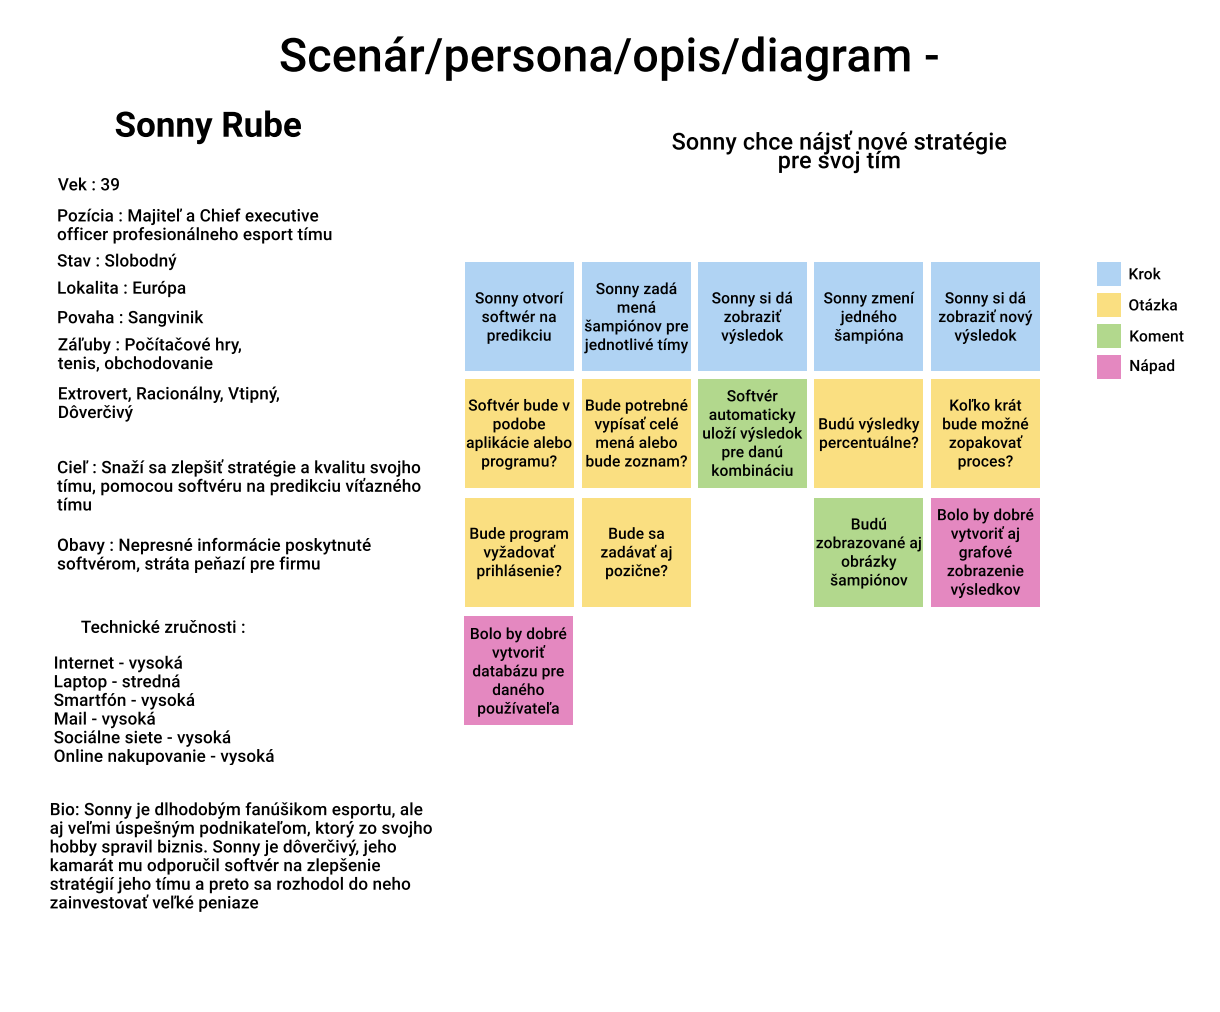
\includegraphics[width=.9\textwidth]{figures/scenar}
	
	\centering
	
	\caption{ Informácie o používateľovi \label{scenar}}
	
\end{figure}

\subsection{Návrh postupností obrazoviek}

Návrh postupností obrazoviek máme rozdelený na 5 častí, podľa nás najdôležitejších častí, ktoré sú nevyhnutné na správny chod, konkrétne obrazovky sú na obrázku \ref{jednanula}. V nasledujúcich častiach si ich predstavíme.
\begin{enumerate}
\item Prihlasovanie

Na prvej obrazovke sa nachádza prihlasovanie do účtu s možnosťou zabudnutého hesla.

\item Prázdna obrazovka

Následné je presunutie na prázdnu obrazovku, kde je potrebné vyplniť miesta na vypočítanie pravdepodobnosti daného tímu na výhru.

\item Vyplnená obrazovka

Potrebujeme vyplniť všetky prázdne políčka šampiónmi z hry League of Legends.

\item Výsledková obrazovka

Po vyplnení môžeme stlačiť tlačidlo vypočítať, ktoré v praxi zoberie zadané tímy a pošle ich umelej inteligencii, ktorá vypočíta percentuálnu výhru obidvoch tímov. Výsledky z tohto pokusu môžeme uložiť.

\item História

To nás automaticky prenesie na ďalšiu obrazovku histórie. V histórii si môžeme prezrieť predošlé vykonané pokusy a ich podrobnosti. Z histórie možeme následne rovno prejsť na nový prípad.
\end{enumerate}
\begin{figure}[h!]
	
	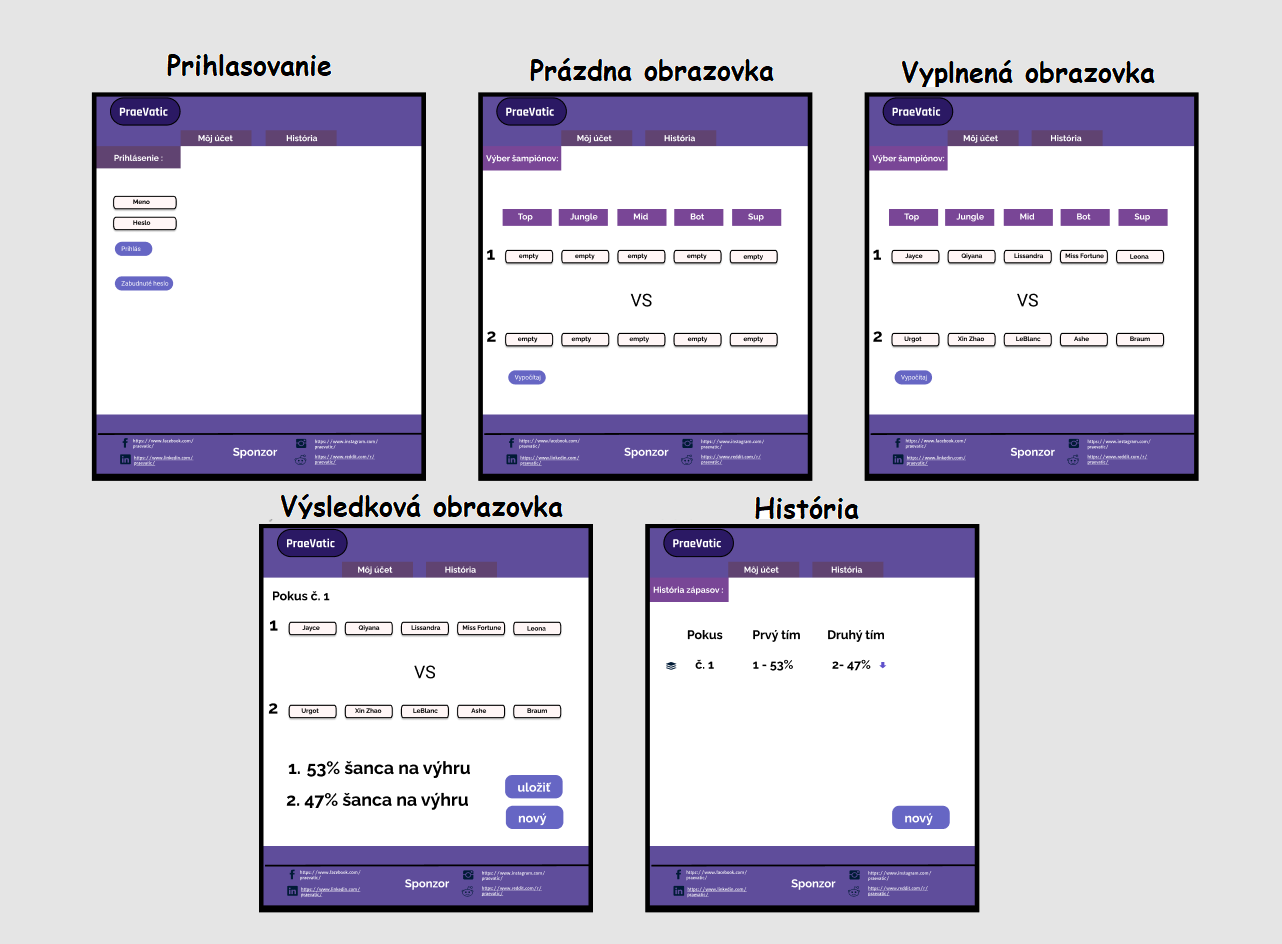
\includegraphics[width=.9\textwidth]{figures/postupnost}
	
	\centering
	
	\caption{ Postupnosť obrazoviek prototypu z nástroja figma \label{jednanula}}
	
\end{figure}

\subsection{Prvý prototyp}

Aktuálny prototyp v nástroji figma\footnote{https://www.figma.com/proto/ze1H0AqlBQMaAQzBSOqKDf/UX-odovzdavky?node-id=2\%3A2\&starting-point-node-id=2\%3A2\&scaling=min-zoom} si môžete prezerať.  
Takisto bolo natočené video \footnote{https://www.youtube.com/watch?v=2UFsyUZgpUM\&t=11s} s ukážkou vykonanie scenárov.
\\ \\
Pri prvom prototype sme použili všetky informácie, ktoré sme objasnili pri prvých bodoch ako scenár. Hlavná bola použiteľnosť a jednoduchosť použitia softvéru na predikciu. Kolorizácia je okolo fialovej farby typ monochromatic. Používateľské testy boli až po vytvorení prvého prototypu. 


\begin{figure}[h!]
	
	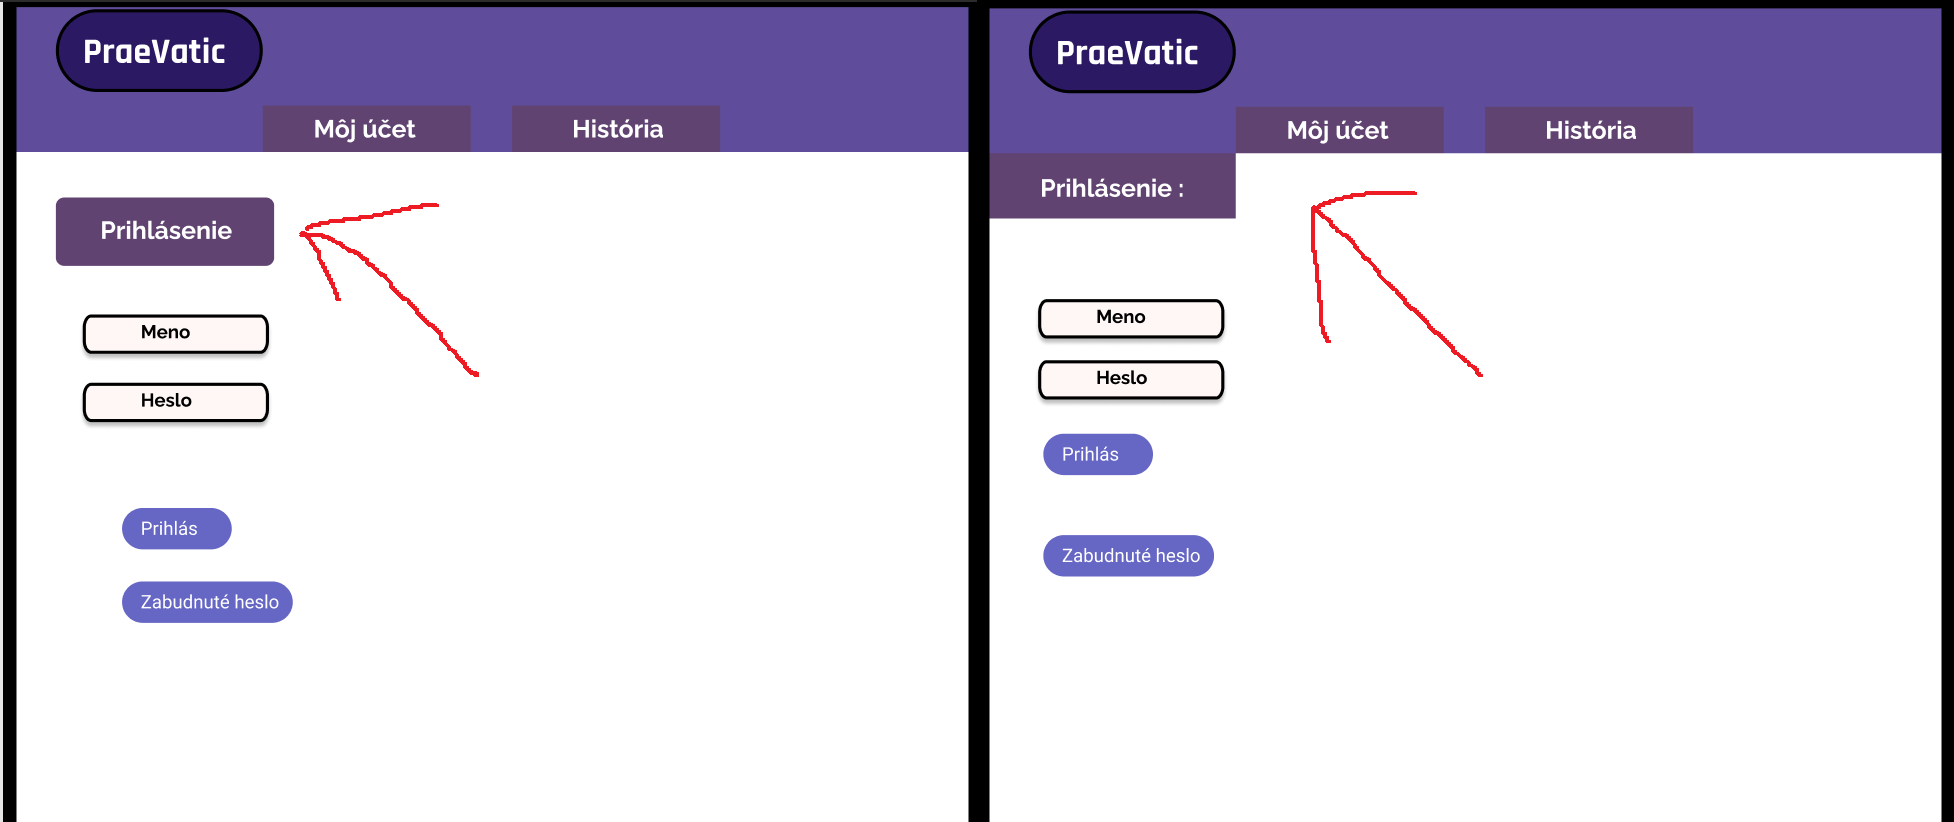
\includegraphics[width=.9\textwidth]{figures/predtym}
	
	\centering
	
	\caption{ Ukážka prvej zmeny v prototype na prihlásenie\label{predtym}}
	
	
	
\end{figure}


Testeri sa pri pokyne prihlásiť sa pokúšali stlačiť fialový nadpis Prihlásenie, to ale nebolo možné a pravdepodobne to bolo mätúce. Preto sme sa rozhodli ho pripojiť k hornej časti a zmeniť oblé okraje. Zmenu je vidno na obrázku : \ref{predtym}


\begin{figure}[h!]
	
	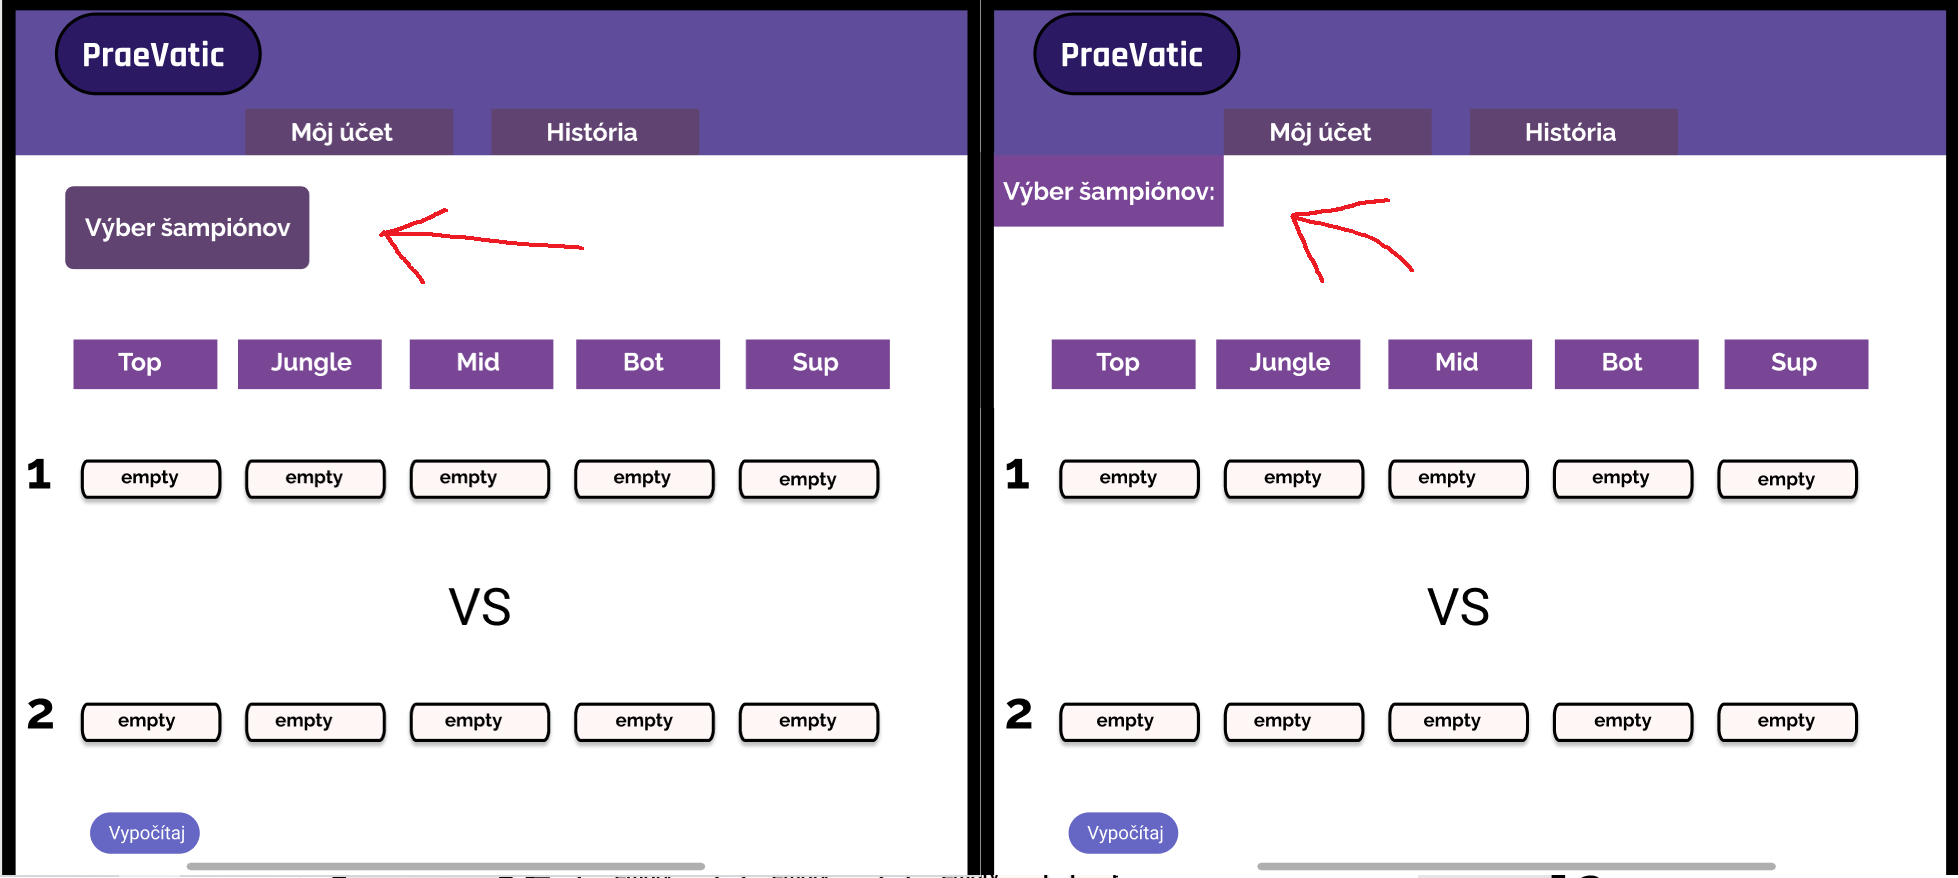
\includegraphics[width=.9\textwidth]{figures/2}
	
	\centering
	
	\caption{Ukážka zmeny v prototype na výber šampiónov\label{2}}
	
\end{figure}

Podobne ako pri prvej zmene sa testeri pokúšali vybrať šampiónov pomocou nadpisu Výber šampiónov, tak sme ho presunuli k okraju, zmenili farbu a zrušili oblé okraje, ako môžeme vidieť na obrázku : \ref{2} 

\begin{figure}[h!]
	
	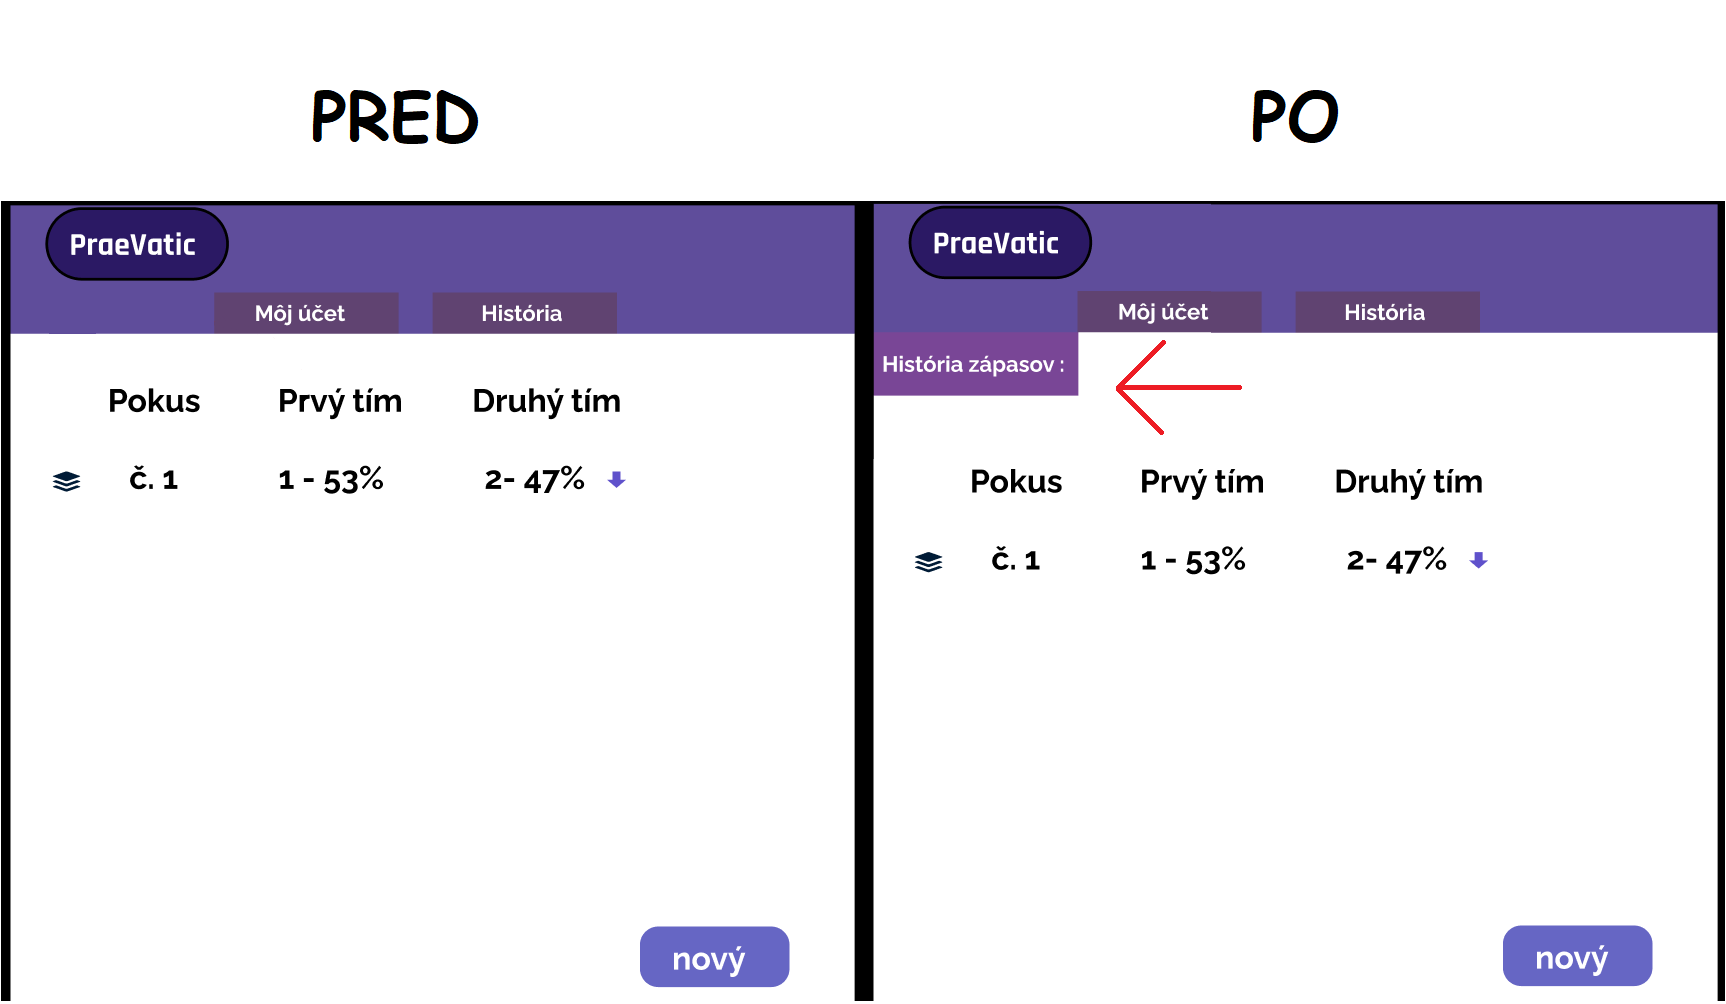
\includegraphics[width=.9\textwidth]{figures/3}
	
	\centering
	
	\caption{ Ukážka zmeny pri histórii zápasov \label{3}}
	
\end{figure}

Na stránke histórie nebolo testerom hneď jasné, o čo sa jedná, tak sme sa rozhodli pridať popis História zápasov na objasnenie, ako vidíme na obrázku \ref{3}.
\\



\begin{figure}[h!]
	
	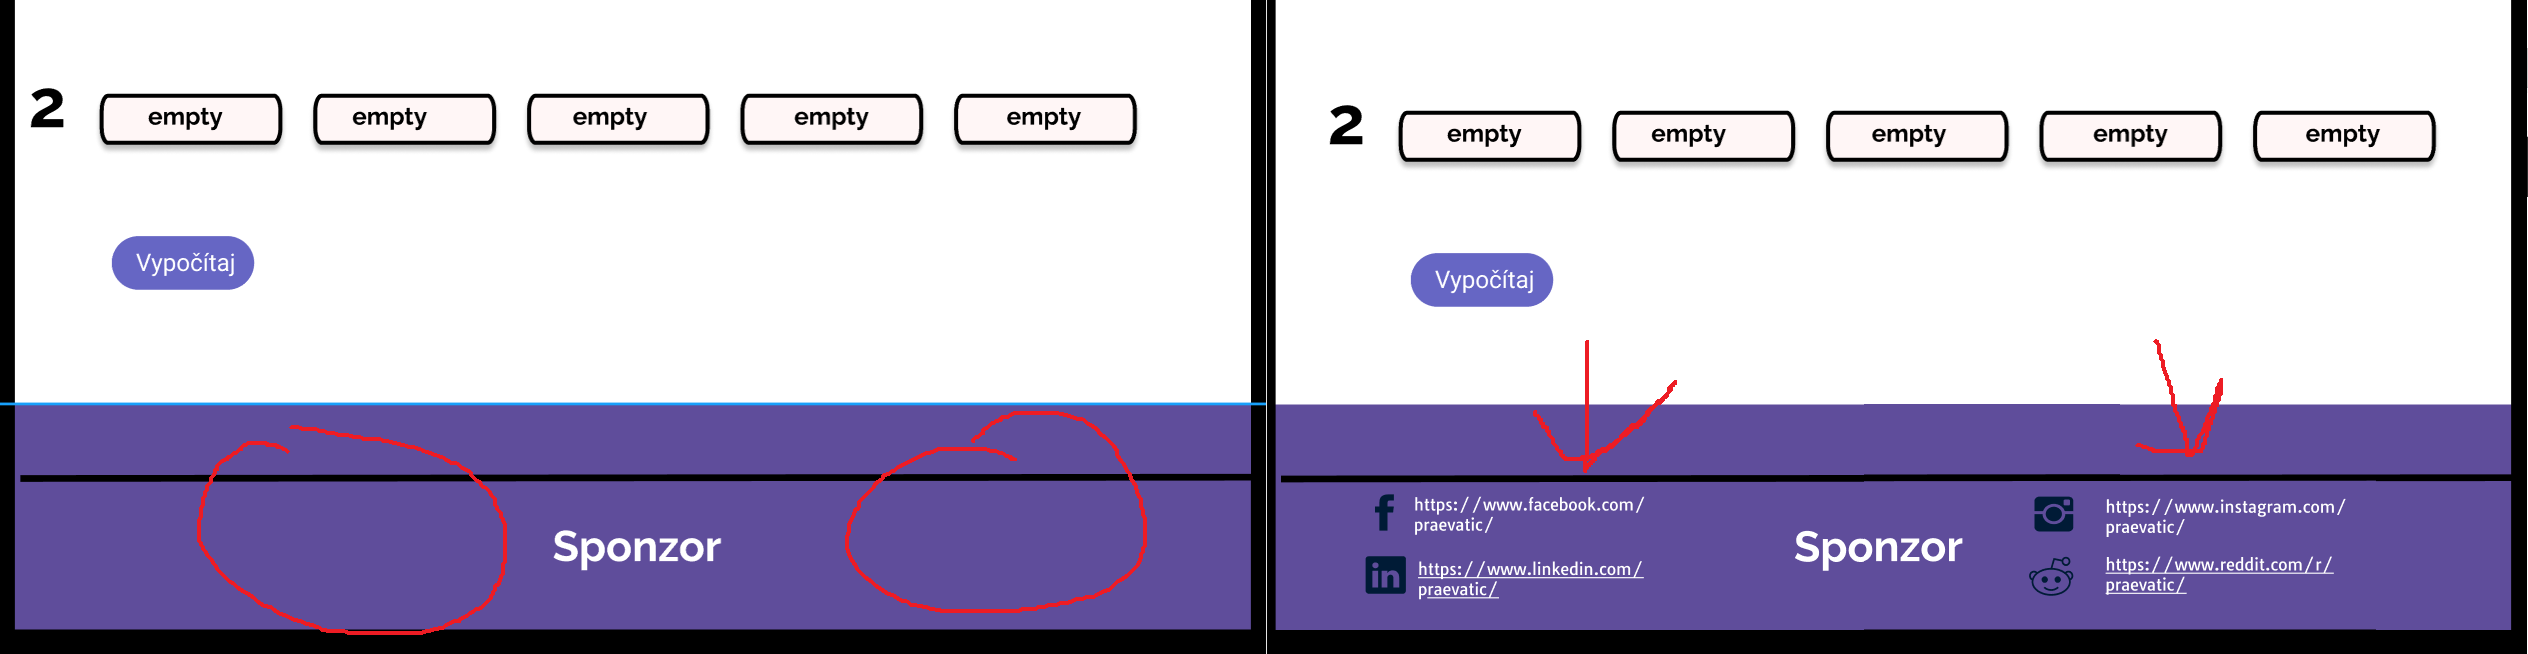
\includegraphics[width=.9\textwidth]{figures/4}
	
	\centering
	
	\caption{ Pridanie sociálnych sietí \label{4}}
	
\end{figure}

Kedže by bolo vhodné mať kontakt so zákazníkmi, aby mali možnosť sledovať zmeny alebo sa zapájať do debát s inými používateľmi, boli pridané sociálne siete\ref{4}, ktoré sú vhodným prostriedkom.





\subsection{Overenie prvého prototypu}



Účastníci hlavného testu boli 4 hráči, ktorí majú nahraté aj hry spomínané v tejto bakalárskej práci. Sú to 3 študenti, z toho 2 vysokoškoláci a 1 maturant a jeden pracujúci. Výsledky SUS dotazníka spomedzi účastníkov boli priemerne 95/100, čo je asi dôsledkom malého počtu účastníkov a zároveň aj vysokej jednoduchosti použitia. Aj keď výsledky SUS boli povzbudzujúce a utvrdili teóriu jednoduchosti používania, nevyšli z nich žiadne praktické výsledky. Na konkrétne podstatné zmeny bolo určené interview a zároveň pozorovanie účastníkov pri vykonávaní scenárov. Bolo potrebné urobiť viacero štylistických zmien na zlepšenie viditeľnosti niektorých popisov, ktoré pripomínali tlačidlá, takisto niektoré prechody a celkovú čitateľnosť. Vykonávanie scenárov a prvé dojmy účastníkov sú zaznamenané a uložené.

\section{Vylepšenie a prepis výsledkov do pochopiteľnej formy pre zákazníka}
V tejto časti sa pokúsime výsledky z predošlých častí dať do roviny celého tímu a zároveň zlepšiť formu, v ktorej sú výsledky prezentované.

\subsection{Výpočet všetkých pozícií}
Vzhľadom na  fakt, že máme 5 šampiónov v tíme, potrebujeme vzťahy každého ku každému. To je dôvod, prečo sme potrebovali nielen dáta miery výhry, ale aj počet hier v daných inštanciách. Použijeme na to 10 dočasných premenných typu bot.games\footnote{bot.winrate = počet hier vypočítaných spočítaním všetkých hier, všetkých 4 tried, s ktorými daný šampión hral} a bot.winrate\footnote{bot.winrate = miera výhry vypočítaná spočítaním priemerných mier výhier všetkých 4 tried, s ktorými daný šampión hral}). Všetkých 5 premenných .games a .winrate spočítame a premennú totalwinrate \footnote{totalwinrate = všetky miery výhier spočítané dokopy}vydelíme premennou totalgames\footnote{totalgames = celkový počet hier}.

\subsection{Forma výsledkov}
Pri hlbšom uvažovaní a hlavne testovaní prototypu sme si uvedomili, že sme nepracovali priamo na určení miery výhry, ale na určovaní kvality kompozície tímu. Preto sme sa rozhodli určovať známky tímovým kompozíciám, ktoré si vyberú profesionálne tímy a na základe toho, akú známku dostanú, určiť pravdepodobnosť na ich výhru oproti tímu s inou alebo tou istou známkou.

\subsection{Známkovanie}
Známky sme sa rozhodli určovať v 8 kategóriach od S+ po F vzhľadom na skóre, ktoré dostanú v premennej totalwinrate, ktoré berie do úvahy vzťahy všetkých šampiónov v kompozícii :  
\begin{enumerate}
	\item Trieda S+ - tu sú zaradené tímy, ktorých kompozícia je vynikajúca, priam neporaziteľná pre všetky neprofesionálne tímy a zároveň tímy so známkou B a nižšie. Ak tím prehrá s touto známkou, muselo sa niečo veľmi pokaziť počas hry, či už veľa smrtí počas začiatku ale aj v strede hry a zároveň musel mať nepriateľský tím tiež veľmi dobrú známku S a lepšie. Tímy dostanú známku S+ pri hodnotení 54,5 a viac. 
	\\ \\ Príklad tejto kompozície je napríklad tím T1 na turnaji MSI 2022 proti tímu SGB. Kde hrali gwen, ktorá slúžila na stranách ako rozptýlenie, ktoré ak si nikto nevšímal, tak zaplatili vysokou cenou, keď ju chceli zastaviť potrebovali na to aspoň dvoch nepriateľských šampiónov, čo otvorilo nové možnosti pre jej tím na druhej strane mapy. Preto mali na pozícii MID Twisted Fate, ktorý sa veľmi ľahko pohybuje po celej mape a môžu ľahko zaútočiť na ostatné strany mapy. Táto kompozícia dostala známku 55,2542 a tím SGB porazila za 23 minút.
	\\
	\item Trieda S  - dostať známku S je takisto veľmi náročné, aj keď rozdiel medzi S a S+ je viditeľný. Tím so známkou S by nemal mať žiaden problém poraziť hocijaký tím so známkou C a nižšie. Ak by hral proti tímu so známkou B alebo A je možné, že pri väčších chybách hru môže prehrať, takisto sa môže stať, že oveľa lepší tím dostane známku A alebo B a skúsenosti toho tímu budú dostatočné na porazenie tímu S. Tímy dostanú známku S pri hodnotení 53,5 až 54,5.
	\\ \\Dobrou ukážkou tímu hodnoteného známkou S je RNG, ktorí na turnaji MSI hrali proti G2esports a porazili ich tím hodnotený známkou D za 26 minút. Ich cieľ hry bolo sústredenie sa na spodnej časti mapy a ochrana ich šampióna na pozícii ADC, ktorý bol v neskorších fázach hry nezastaviteľný. Ich tím bol hodnotený skóre 54,1329
	\\
	\item Trieda A  - známka A je stále ťažko dosiahnuteľná pre väčšinu tímov, keďže na jej hodnotenie je potrebné hlbšie poznanie šampiónov a ich synergií. Ak tím dostane známku A, malo by byť preňho jednoduché pochopiť plán danej kompozície, nie vždy musí byť realizácia jednoduchá, ale mala by byť uskutočniteľná. Tieto tímy môžu mať problémy s tímami so známkou A alebo B, no nemali by mať žiadne problémy proti tímom so známkou D a horšie. Tímy dostanú známku A pri hodnotení 52,5 až 53,5.
	\\  \\Príklad kompozície typu A je napríklad tím EG na turnaji MSI2022 proti tímu ORDER, kde na pozícii MID hrali Ahri, ktorá ľahko naláka nepriateľov a tým, že na pozícií JG bol Xin Zhao, ktorý je veľmi silný v ranných štádiach hry, tak veľmi ľahko dostali náskok a nepriatelia ich už nedokázali zastaviť.
	\\
	\item Trieda B  - najväčšia časť profesionálnych tímov dostane známku B. Sú to na profesionálnej scéne priemerné alebo mierne nadpriemerné kompozície, ktoré môžu, ale často neprekvapia. Ich cieľ môže byť predvídateľný, čo môže spôsobiť ich nižšiu šancu na výhru. Môžu poraziť tímy so známkou A alebo S, no bolo by to veľmi náročné. Na druhej strane by nemali mať najmenší problém poraziť tímy E alebo F. Tímy dostanú známku B pri hodnotení 51,5 až 52,5.
	\\ \\
	Príklad tejto kompozície je napríklad tím G2Esports na turnaji MSI 2022 proti tímu ORDER, kde hrali gnara na pozícii TOP, jeho prioritou je udržiavanie nepriateľov na jeho strane, získavanie veží a CC počas tímových súbojov. Na pozícií JG hrali wukonga, ktorého úlohou je počas tímových súbojov udržiavať nepriateľov na jednom mieste. Na pozícií MID hrali Leblanc, ktorej úlohou je assasinácia nepriateľských slabších článkov. Na pozícii bot hrali zeri, ktorá má vysokú mobilitu\footnote{mobility = pohyblivosť na mape} a ľahko a rýchlo sa dostane do tímového súboja. Na pozícii SUP hrali Renata Glasc, ktorej úlohou je posilňovanie jej celého tímu a takisto udržanie nepriateľov na jednom mieste. Táto kompozícia dostala hodnotenie 52,1026. 
	\\
	\item Trieda C  - druhá najväčšia časť tímov dostáva známku C. Pri profesionálnych tímoch je to presný priemer. Plán, ktorým tím disponuje, je prehliadnuteľný, najlepšie tímy ako S a S+ nemá skoro žiadnu šancu poraziť. No tímy so známkou A alebo B môže poraziť, ak by robili viacero chýb. Tento tím  by nemal mať žiaden problém poraziť tím typu F. Tímy dostanú známku C pri hodnotení 50,5 až 51,5.
	\\ \\ Dobrým príkladom by bola hra tímu Istanbul Wildcats, ktorý porazil tím RED Canids, hodnotený známkou D, za 28 minút. Na pozícii MID mali Ahri, ktorá sa ľahko pohybuje po mape a tým, že mali na pozícii SUP nautilusa, ktorý vie ľahko chytiť nepriateľa a na chvíľu ho udržať na mieste, tak mali dobrý a celkom efektívny plán na zabitie nepriateľov. Ich tím bol ohodnotený skóre 51,0694.
	\\
	\item Trieda D  - ak profesionálny tím dostane známku D, musel byť zahnaný do kúta a nemal na výber šampiónov, ktorých chcel vybrať, keďže pri fáze výberu tímu môže nepriateľský tím zabanovať\footnote{zabanovať = odstrániť šampióna z celkového výberu v danom zápase} 5 šampiónov. To ale neznamená, že aj tento tím nemá možnosť poraziť silnejšie tímy, a to konkrétne tímy so známkou B, C a malú časť A tímov. Tímy dostanú známku D pri hodnotení 49,5 až 50,5.
	\\ \\ Ako príklad sa pozrieme na hru medzi tímom Detonation FocusMe a Team Aze, kde po veľmi náročnej hre, ktorá trvala 37 minút, Team Aze vyhral s hodnotením D nad tímom so známkou A. Ich kompozícia nebola najideálnejšia, keďže na pozícii BOT mali Ezreala, ktorý nedáva zmysel, keďže všetci ostatní členovia tímu sa hrnú dopredu a snažia sa čo najrýchlejšie zabiť nepriateľa, pričom Ezreal chce z diaľky a postupne ostreľovať. Ich tím bol ohodnotený skóre 50,3936.
	\\
	\item Trieda E  - pri známke E pre profesionálne tímy nie je veľa výhovoriek, nemalo by sa to diať. Sú to väčšinou kompozície, ktoré nemajú jasný plán a šampióni nekomplimentujú seba navzájom. Pre typ tohto druhu je veľmi ťažké poraziť hocijaký tím so známkou lepšou ako C. Tímy dostanú známku E pri hodnotení 48 až 49,5.
	\\ \\
	Veľmi dobrým príkladom je hra medzi tímom G2Esports a Saigon Buffalo. G2Esports je na papieri oveľa silnejší tím a nemal by mať problém poraziť Buffalo. Ale náš program ohodnotil tímovú kompozíciu G2 na D a Buffalo na známku S. Hra skončila za 26 minút a G2 prehrali. Ich šampióni boli síce osamote veľmi silní, ale dokopy nedávali zmysel a to sa preukázalo v tímových súbojoch, kde vôbec nevedeli, čo majú robiť. Ich tím dostal skóre 48,8665.
	\\
	\item Trieda F  - veľmi málo profesionálnych tímov dostane známku F. Sú to tímové kompozície, ktoré spolu vôbec nedávajú zmysel, nemajú plán, ktorý sa dá zrealizovať a hru môžu vyhrať len veľkou náhodou a to len proti tímom so známkou F alebo E. Tímy dostanú známku F pri hodnotení 48 a nižšie.
	\\ \\
	Dobrým príkladom je tímová kompozícia tímu ORDER proti G2 na turnaji MSI2022, prehrali za 26 minút proti kompozícii ohodnotenej B. Kombinácia ich šampiónov vôbec nedávala zmysel, každý šampión sa vo svojej podstate snažil o niečo iné, čo dospelo k úplnému rozpadu ich tímu. Tým si zaslúžili známku F za celkové skóre 46,2914.
	\\
\end{enumerate}


\subsection{Implementácia testovania}
Testovanie bolo vykonané na skupine 58 zápasov. Pri testovaní sme použili náš program, kde sme vložili všetkých 116 rôznych tímových kompozícií. Obidvom tímom bolo priradené skóre a zároveň aj ohodnotenie ich kompozície známkou. Pri každom tíme je takisto aj počet všetkých rôznych kombinácií, v ktorých sa daný šampióni stretli. Spracovanie výsledkov bude v nasledujúcej časti vyhodnotenia.
